\documentclass{article}
% option ``report'' puts title on separate page

\usepackage{amsmath}
\usepackage[pdftex]{graphicx}

\begin{document}

\title{WS4: ODE Integration: Simplified Stellar Structure}
\author{Jackie Villadsen}
\date{\today}
\maketitle


\section{Structure of a White Dwarf}

\begin{figure}[h]
  \begin{center}
     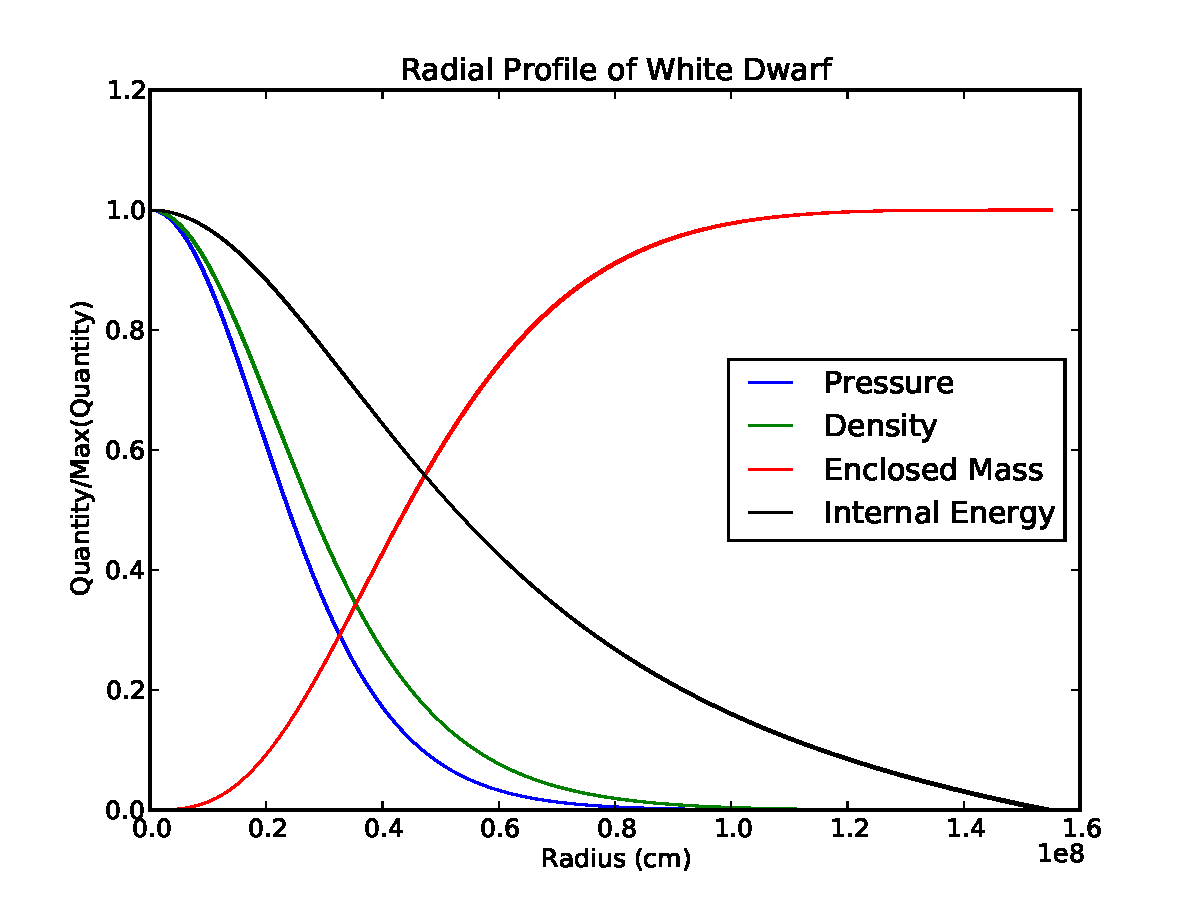
\includegraphics[width=\textwidth]{radial}
  \end{center}
  \caption{The radial profiles of pressure, density, enclosed mass, and internal energy of a fully
relativistic white dwarf.  All quantities are renormalized to have a maximum of 1.}
  \label{fig:radial}
\end{figure}

The framework provided for integrating over the structure of a white dwarf uses Runge-Kutta integration.
The main code loops over a range of numbers of integration steps, then calls a function that 
integrates to obtain the mass and radius of the white dwarf using the given number of integration steps.
This integrator function first calls a function that sets up the radial grid, and defines the central pressure
and enclosed mass (at step 0).  It then performs a loop where it calls a Runge-Kutta function that uses
the current values for radius, enclosed mass and pressure to call a function that evaluates the derivative (the
right-hand side) and then uses that derivative and perhaps derivatives at intermediate steps, depending on the order,
to step forward one step in the radial grid.  At each step the density and internal energy are also evaluated.
The result is that every time the overall integration function is called,
it returns the radial profile of the pressure, density, enclosed mass, and internal energy of the star.  These
results are shown in Figure \ref{fig:radial}.

The star is a relativistic white dwarf, so $\Gamma = 4/3$, and the mass follows the Chandrasekhar mass limit.
For 4th-order Runge-Kutta and 100,000 integration steps, I obtain R = 1551 km and M=1.457$M_\odot$.

\section{Convergence}

\begin{figure}[h]
  \begin{center}
     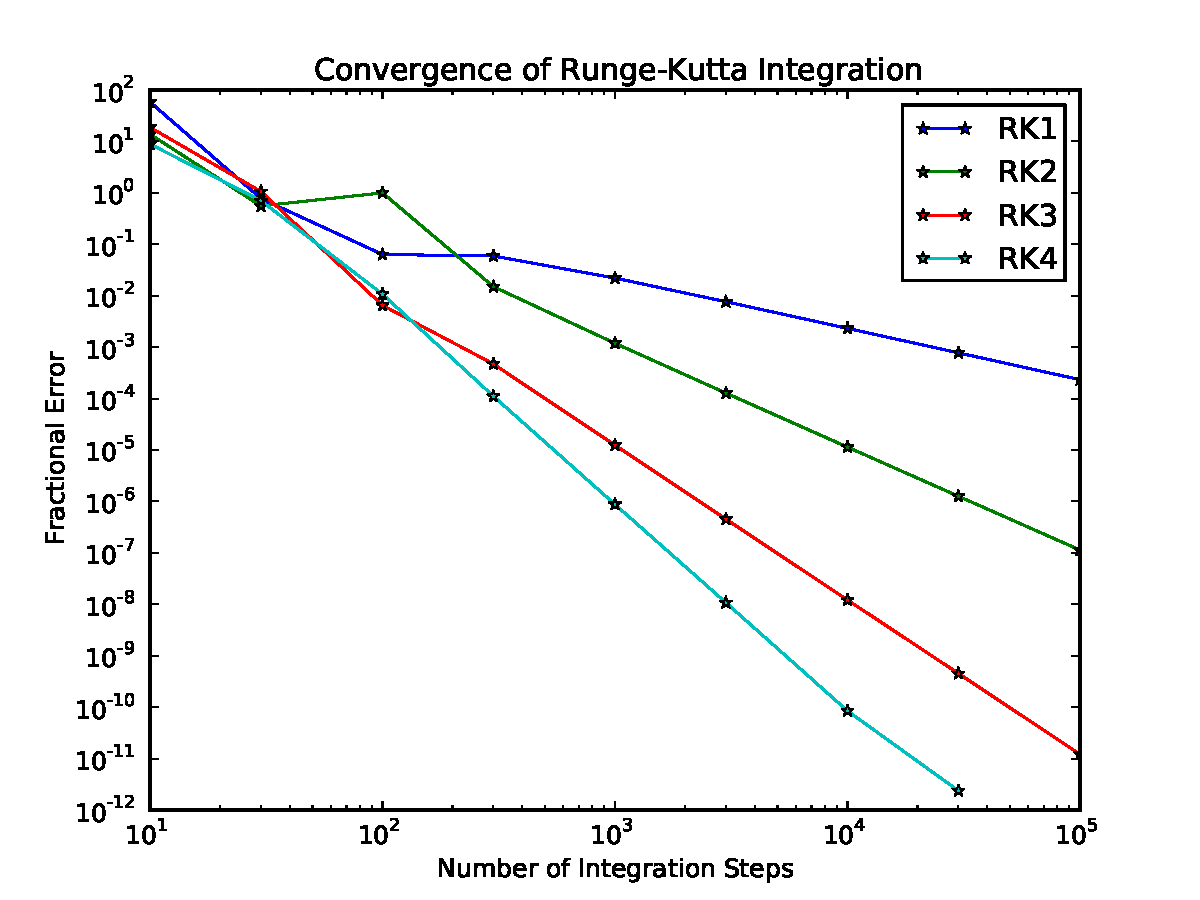
\includegraphics[width=\textwidth]{rk}
  \end{center}
  \caption{Fractional error on the mass for Runge-Kutta integration schemes of first through fourth order, versus
the number of integration steps.  On a log-log plot, a scheme of order n has a convergence slope of -n.}
  \label{fig:rk}
\end{figure}

To calculate the convergence of the different orders of Runge-Kutta, I took the result for the mass from 4th-order
Runge-Kutta with 100,000 integration steps (the most I used) to be the ``answer.''  I then compared the
fractional error compared to this answer for the results from Runge-Kutta of orders 1 through 4 with 
numbers of integration steps ranging from 10 to 100,000.  Figure \ref{fig:rk} shows the fractional
errors for each different order of Runge-Kutta on a log-log plot.  Since it is on a log-log plot,
and number of integration steps is the inverse of dr, then an nth order Runge-Kutta (O(n)) will have
a slope of -n.  On the plot we see that this is true, which I confirmed by printing the log of the ratio
of two fractional errors (same order RK) over the log of the ratio of the corresponding numbers of steps.

\end{document}